\section{Summarized Experimental Results}\label{sec:ExperimentalResults}
This section summarizes the issues and results of the experiments, sorted by topic. In total around 17 different experimental sessions were recorded and analyzed. The earlier tests in which the experimental structure was not yet established are not included. All relevant sessions are briefly documented and included in the appendix. Their calibration patterns and examples of the image sequences are in the digital content. The last section describes the most successful experiment in greater detail (\autoref{ssec:Session14}).

%------------------------------------------------%
% Time
%------------------------------------------------%
\paragraph{Time.}
The calibration takes a long time and the cameras must not be moved at all during the entire process. Only after all necessary calibration images are captured can the success or failure of the calibration process be verified. In many sessions the calibration had to be repeated, sometimes because the cameras were moved by accident and sometimes because of a failed calibration in MATLAB.

%------------------------------------------------%
% Cam set-up	
%------------------------------------------------%
\paragraph{Illumination vs. depth of field.}
The high-speed cameras need a lot of light due to their high frame rate. By keeping the cameras' aperture as wide open as possible one can maximize the efficacy of the lighting, but this results in a very narrow depth of field, causing blurred images and making the calibration process extremely difficult. The checkerboard needs to be moved to different angles in order to get a satisfactory amount of calibration images, but this is hard to achieve when the depth of field is too narrow. Adding more lights results in in reflections on the objects and checkerboards which can also lead to calibration errors.

The early experimental sessions were too dark or the objects out of focus. The best results could be achieved with an aperture of 8, 4 LEDs and a distance of about 1,5 m between the cameras and the objects of interest.

\paragraph{Baseline and camera position.}
Several camera positions were tested to achieve the best results. In the first sessions (number \textit{1} to \textit{3}) the cameras were set-up on two different camera tripods with a relatively large baseline. The cameras were not parallel to each other. In \textit{session 4} the two cameras were set parallel to each other, but still with a relatively large baseline, since they were still on two separate tripods. The baseline in \textit{session 9} was decreased which resulted in more images pairs being accepted by the camera calibrator but still did not improve the process. From \textit{session 13} onward the cameras were placed on a rig and as parallel to each other as possible. The form of the camera case and the cables still result in a baseline between 15 to 20 cm.

\paragraph{Hardware problems}
The cameras disconnected several times after which the TimeBench software and sometimes even the computer had to be restarted which was quite time-consuming. In a few sessions the cameras produced black images.

%------------------------------------------------%
% Cam calibration
%------------------------------------------------%
\paragraph{Problems with the checkerboard.}
The checkerboard detection is the most important process for the camera calibration. Next to the time-consuming factor, the checkerboard was the cause of many problems. In the early sessions (\textit{1-5}) a big checkerboard in the size of a DIN A4 paper was used. The small depth of field often resulted in checkerboard images that were out of focus, or even out of frame. The lighting was challenging as well: too much and the reflections ruined the images, too little and the images became too dark to be able to be calibrated. By limiting the checkerboard to fewer squares (in \textit{session 2}) and editing the images in \textit{Photoshop}\footnote{The contrast was increased and disturbing artifacts were masked.}, more image pairs were accepted by the Stereo Camera Calibrator. Stereo camera calibration creates another problem: if one checkerboard image is unreadable its corresponding pair image is rendered useless as well, this results in far fewer images pairs being accepted.

\textit{Session 6} used a smaller checkerboard, which was easier to handle but was printed at a low quality. The tape used to attach the checkerboard to the paper reflected too much light and the square were not clean enough. The process of capturing the calibration images was improved by recording the calibration sequence in a lower frame rate (50-80 fps) in \textit{session 11} which allowed more time to move the checkerboard pattern to different angles.

\textit{Session 12} introduced an even smaller checkerboard which was printed professionally and which had a much smoother surface. This final checkerboard had the ideal form and improved the calibration process. The square size was now 3 mm.

\paragraph{Objects to be reconstructed}
There were different objects of interest involved in the experiments. In \textit{session 1 to 11} simple toy blocks were pushed over with a toy car. In several sessions different moving objects like a balloon (\textit{session 4}) or a toy magic wand (\textit{session 3}) were captured as well. Since the feature detection algorithms need as many different features as possible, the symmetric toy blocks were first altered with graffiti stickers (\textit{session 12}) and then completely exchanged with asymmetrical objects (\textit{session 13}).    

\paragraph{Rectification}
The biggest problem in the camera calibration process was and still is, the image rectification. The rectified images are either black or do not have the correct size. Changing the cameras' position, adding more image pairs or improving the overall image quality did not change the result. The fundamental matrix computed by the Stereo Camera Calibrator seems to be incorrect. A test with normal \textit{SLR} cameras in \textit{session 13} was successful. In \textit{session 14} the rectification finally worked out fine (a discussion of this session can be found below). After this session it seemed like the error occurred when the cameras were not parallel to each other and when the baseline was too large. A later session (\textit{17}) with almost the same set-up disproved this theory. To this date it is still unclear what causes this error. Several forum posts mention similar problems but the given answers could not be applied to this situation. Solutions were: adding more image pairs and reducing the projection error by deleting outliers. All this is not relevant in these experiments since enough image pairs are accepted and the mean error is way below the recommended maximum.

\subsection{Session 14}\label{ssec:Session14}
Session 14 is the only session in which the rectification works perfectly with the footage of the high-speed cameras. The cameras were placed on a rig parallel to each other with almost no rotation and a baseline of about 20,7 cm. The cameras were triggered with an external trigger with the option \textit{falling edge}. The checkerboard's squares had the size of 3 mm and the images for calibration were captured with the help of an image sequence at 70 fps.

The actual image sequences were captured at 500 fps. Additionally several still images were taken. Although only 7 out of 19 image pairs were accepted in the Stereo Camera Calibration the rectification was successful. \autoref{fig:session1417Rectify} shows the comparison between the successful rectification of session 14 and the corrupted one of session 17 which had a very similar camera set-up.

\begin{figure}[htbp]
		\centering
		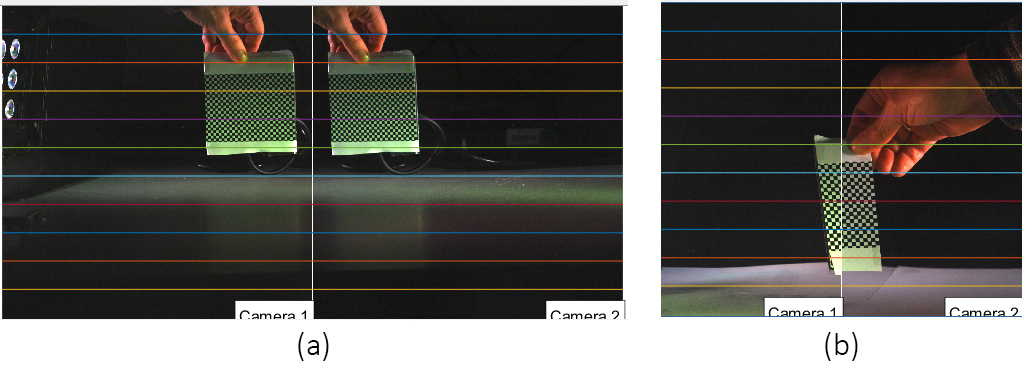
\includegraphics[width=0.8\textwidth]{figures/RectifyCompared}
		\caption[Comparison of the rectification of session 14 and 17]{Comparison of the rectification of \textbf{session 14} and \textbf{session 17}.}
		\label{fig:session1417Rectify}
\end{figure}

The extrinsic camera parameters are computed correctly (see \autoref{fig:session14Extrinsics}) and the overall mean error is with 0.11 very low.

\begin{figure}[htbp]
		\centering
		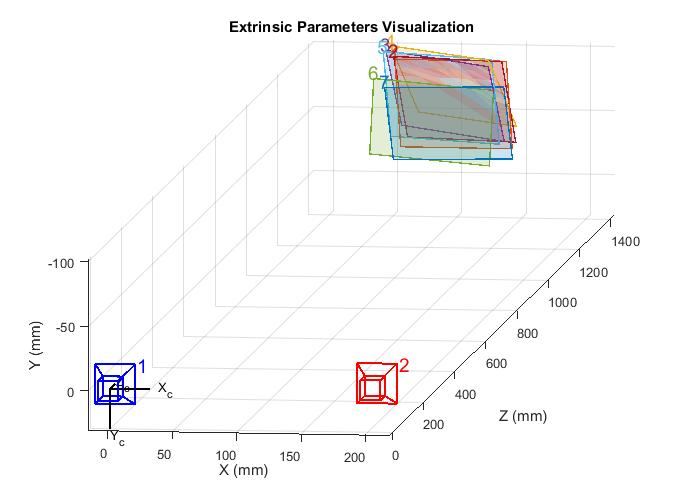
\includegraphics[width=0.8\textwidth]{figures/ExtrinsicParams}
		\caption[Extrinsic parameters of session 14]{Extrinsic parameters of session 14.}
		\label{fig:session14Extrinsics}
\end{figure}

The scenes were reconstructed smoothly. The car was the most difficult object for the algorithms to recognize. A screenshot of the reconstruction can be seen in \autoref{fig:PointCloud}.